%%%%%%%%%%%%%%%%%%%%%%%%%%%%%%%%%%%%%%%%%%%%%
\section{Distributed angular momenta}
\label{Sec:DistributedL}
%%%%%%%%%%%%%%%%%%%%%%%%%%%%%%%%%%%%%%%%%%%%%

In sections~\ref{Sec:FarFromEq} and~\ref{Sec:Epicyclic} all the gas particles have the same magnitude $L_0$ of the angular momentum. In this section we let the angular momenta be distributed about $L_0$ with the root mean square width $\sigma_L$. The core and its oscillation turn out to require angular momenta which are equal to within about one percent: for $M_{gas}/M = 0.03$ ($\mu = 0.52$), a width $\sigma_L/L_0 = 0.18$ percent changes nothing, a width of $0.71$ percent halves the mass of the core, and a width of $1.41$ percent removes it. The width which is needed grows with the mass of the cloud. The mass which accumulates near the circular orbit is reduced less. The mechanism is the dependence of the orbital frequencies on $L$, which dephases the parts of the core with different angular momenta. We first extend the epicyclic model to distributed angular momenta (section~\ref{SubSec:DistModel}), then describe the PIC simulations (section~\ref{SubSec:DistRuns}), and finally present the results for a fixed mass (section~\ref{SubSec:DistResults}) and their dependence on the mass (section~\ref{SubSec:DistBoundary}).


\subsection{The epicyclic model with distributed angular momenta}
\label{SubSec:DistModel}

When the shells have different angular momenta $L_j$, two of their properties depend on $j$: the frequency $\Omega(J_j,L_j)$ of the radial motion and the radius $R(L_j)$ of the circular orbit about which the shell oscillates. We define the amplitudes $\zeta_j$ by Eq.~(\ref{Eq:zetaDef}) with the same frequency $\kappa_0 = \Omega(0,L_0)$ for all the shells, such that the differences $\Omega(0,L_j) - \kappa_0$ appear as a slow rotation of $\zeta_j$. Replacing $\Omega(0,L_j)$ with $\kappa_0$ in the amplitude of Eq.~(\ref{Eq:Epicycle}), which introduces a relative error of the order of $\sigma_L/L_0$, one finds $\xi_i - \xi_j = D_{ij} - \kappa_0^{-1/2}\re[(\zeta_i - \zeta_j)e^{i\kappa_0 t}]$ with $D_{ij} := R(L_i) - R(L_j)$. The average of $|D - \rho\cos\theta|$ over $\theta$ is $|D|$ when $|D|\geq\rho$, since then the expression inside the modulus does not change its sign, and $(2/\pi)[(\rho^2 - D^2)^{1/2} + D\arcsin(D/\rho)]$ when $|D| < \rho$. Hence, Eq.~(\ref{Eq:AverageFixedL}) is replaced with
\begin{equation}
\left\langle \left| \xi_i - \xi_j \right| \right\rangle = \frac{2}{\pi\sqrt{\kappa_0}}\,\mathcal{G}\left( |\zeta_i - \zeta_j|,d_{ij} \right),\qquad
\mathcal{G}(\rho,d) := \left\{ \begin{array}{ll}
\sqrt{\rho^2 - d^2} + d\arcsin\left( \displaystyle\frac{d}{\rho} \right), & |d| < \rho,\\
\displaystyle\frac{\pi}{2}|d|, & |d|\geq\rho,
\end{array} \right.
\label{Eq:KernelL}
\end{equation}
with $d_{ij} := \sqrt{\kappa_0}\, D_{ij}$. The function $\mathcal{G}$ reduces to $\rho$ for $d = 0$, and it is continuously differentiable with $\partial\mathcal{G}/\partial\rho = (1 - d^2/\rho^2)^{1/2}$ for $|d| < \rho$. The Hamiltonian~(\ref{Eq:Hepi}) becomes
\begin{equation}
\overline{H} = \sum\limits_{j=1}^N m_j\left[ E(J_j,L_j) - \kappa_0 J_j \right] + g\sum\limits_{i<j} m_i m_j\,\mathcal{G}\left( |\zeta_i - \zeta_j|,d_{ij} \right),
\label{Eq:HepiL}
\end{equation}
and the equations of motion are
\begin{equation}
\frac{d\zeta_i}{dt} = i\left[ \Omega(J_i,L_i) - \kappa_0 \right]\zeta_i
 + i g\sum\limits_{j\neq i} m_j\,\frac{\sqrt{\max\{ |\zeta_i - \zeta_j|^2 - d_{ij}^2,0 \}}}{|\zeta_i - \zeta_j|^2}\left( \zeta_i - \zeta_j \right).
\label{Eq:EpicyclicL}
\end{equation}
The spread of the angular momenta has two effects. First, it softens the interaction. Two shells whose circular orbits are separated by more than the amplitude of their relative radial oscillation never cross each other; the force between them is constant in time, and on average they do not exchange energy. When the shells do cross, their interaction is weaker than for equal angular momenta by the factor $(1 - d_{ij}^2/|\zeta_i - \zeta_j|^2)^{1/2}$. Second, the first term on the right-hand side of Eq.~(\ref{Eq:EpicyclicL}) now depends on $L_i$, which produces a differential rotation between shells with the same action variable; the mixing which it causes in the absence of self-gravity has been analyzed in Ref.~\cite{pRoS20}. For the isochrone potential, $\Omega$ only depends on $J + c(L)$, see Eq.~(\ref{Eq:OmegaIsochrone}), and with $L_0 = 2$ one has $R'(L_0) = 4.183$, $c'(L_0) = 0.854$ and $|\partial\Omega/\partial L| = 0.0754$ at $J = 0$.

The core is more sensitive to these effects than the cloud as a whole, because it is small and because the frequencies associated with it differ little from each other. For $M_{gas}/M = 0.02$ its root mean square radial extension is $0.15$, and the frequencies of its particles exceed the frequency of its oscillation by about $9\times 10^{-4}$ (Table~\ref{Tab:ModelFrequencies}). The spread $R'(L_0)\sigma_L$ of the circular orbits reaches the extension of the core for $\sigma_L = 0.036$, whereas the spread $|\partial\Omega/\partial L|\sigma_L$ of the frequencies of the circular orbits reaches $9\times 10^{-4}$ already for $\sigma_L = 0.012$, that is, for $\sigma_L/L_0 = 0.6$ percent. Therefore, the core is expected to be lost when $\sigma_L/L_0$ is of the order of one percent, mainly through the spread of the frequencies.

The model omits a term which only matters for distributed angular momenta. The uniform force of Eq.~(\ref{Eq:PairExpansion}) shifts the frequency of each shell by the amount~(\ref{Eq:UniformShift}), with the mass which the shell encloses on average. For equal angular momenta this shift is the same for all the shells, but for distributed ones it is not: a shell with a larger value of $L$ encloses more mass, which raises its frequency and counteracts the decrease of $\Omega$ with $L$. In a test with two shells whose circular orbits differ, the relative phase of the shells advances $1.8$ to $6.0$ percent faster in the model than in the exact solution, and only $0.4$ to $1.5$ percent faster when this term is included. Evaluated on the solutions of the model, it would reduce the differential rotation between shells with different $L$ by $5$ to $11$ percent for $M_{gas}/M = 0.03$ and by $2$ percent for $M_{gas}/M = 0.01$, for $t\geq 10\tau_1$. Hence, the cores of the PIC simulations should be somewhat more resistant to the spread of the angular momenta than those of the model.


\subsection{Simulations}
\label{SubSec:DistRuns}

For distributed angular momenta we use a second implementation of the PIC method of section~\ref{SubSec:PIC}, in which each computational particle carries its own angular momentum $L_j$. With equal angular momenta and the same particles, it reproduces the simulation of the first code with $M_{gas}/M = 0.021$: the functions $|h_1(t)|$ of both codes differ by at most $4.1\times 10^{-7}$ of the largest value of $|h_1|$ up to $t = 5\tau_1$ and by at most $7.2\times 10^{-5}$ up to the end of the simulation, and all the quantities of section~\ref{Sec:FarFromEq} agree to four digits.

The initial datum is the cloud~(\ref{Eq:Pulse}) multiplied with the factor $\exp[-(L - L_0)^2/s_L^2]$, such that $\sigma_L = s_L/\sqrt{2}$, with $L_0 = 2$ in the isochrone potential. The computational particles are placed on the lattice $N_J\times N_Q = 200\times 50$ in $(Q,J)$, without the points whose weight is smaller than $10^{-7}$ of the largest one, and on $N_L$ midpoints of the interval $|L - L_0|\leq 2.5\, s_L$; their masses contain the factor $L$ of the volume element~(\ref{Eq:PSVolumeForm}). The lattice in $L$ produces a spurious recurrence of the layers with different $L$ at the time $2\pi/(|\partial\Omega/\partial L|\,\Delta L)$, with $\Delta L$ the spacing of the lattice. We choose $N_L$ such that, in the absence of self-gravity, the sum of the phase factors $\exp[-i\Omega(J,L)t]$ over the lattice in $L$ differs from the one of the Gaussian distribution by less than $7\times 10^{-4}$ up to the end of the simulation at $t = 10^4$. This requires $N_L = 6$, $8$, $12$, $20$, $30$, $50$, $70$ and $120$ for $s_L = 0.0025$, $0.005$, $0.01$, $0.02$, $0.04$, $0.06$, $0.08$ and $0.12$, respectively; for $s_L\geq 0.08$ the layers with smaller $L$, which rotate faster, require more points than a linear growth with $s_L$ would suggest. The simulations with $M_{gas}/M = 0.01$, $0.02$, $0.03$ and $0.05$ ($\mu = 0.31$, $0.43$, $0.52$ and $0.66$) are listed in Table~\ref{Tab:DistL}. For $s_L = 0$ they use the same lattice in $(Q,J)$, which explains the small differences with respect to the values of section~\ref{Sec:FarFromEq} (for instance, $m_c = 0.217$ instead of $0.232$ for $M_{gas}/M = 0.03$). We have solved Eq.~(\ref{Eq:EpicyclicL}) with the same particles, with a second-order splitting scheme in which the rotation with the frequency $\Omega(J,L) - \kappa_0$ is solved exactly and the interaction is advanced with the midpoint rule, with $\Delta t = 5$; at $t = 10^3$ its solution differs from the one of the Runge-Kutta scheme of section~\ref{SubSec:EpiComparison} by less than $5\times 10^{-4}$ in $\zeta$.

In order to test the convergence, we have repeated the simulation with $M_{gas}/M = 0.03$ and $s_L = 0.02$ with $N_L = 30$ instead of $20$, and with half of the grid spacing. The mass $m_c$ of the core, the fraction of the mass with $J < 0.2\sigma_J$ and the mean of the values of $|h_1|$ of the individual layers of the lattice in $L$ agree to within $3$ percent in the three simulations, and the residual oscillation~(\ref{Eq:deltaPhiNorm}) of the potential to within $15$ percent. The value of $|h_1|$ of the whole gas, however, depends on $N_L$: over $10\leq t/\tau_1\leq 20$ its mean value is $6.7\times 10^{-3}$ with $N_L = 20$ and $3.7\times 10^{-3}$ with $N_L = 30$, because it depends on how finely the spread of the phases of the different layers is resolved. For $s_L > 0$ we therefore regard the values of $|h_1|$ in Table~\ref{Tab:DistL} as upper bounds.

\begin{table}[htp]
\begin{center}
\begin{tabular}{ll|cc|cc|cc|cc}
\hline\hline
 & & & & \multicolumn{2}{c|}{$|h_1|/h_0$} & \multicolumn{2}{c|}{mass with $J < 0.2\sigma_J$} & \multicolumn{2}{c}{$m_c$} \\
$M_{gas}/M$ & $\mu$ & $\sigma_L/L_0$ (\%) & $N_L$ & PIC & model & PIC & model & PIC & model \\
\hline
\TabL
\hline\hline
\end{tabular}
\end{center}
\caption{The cloud~(\ref{Eq:Pulse}) with distributed angular momenta: PIC simulations and epicyclic model with the same particles. Mean value of $|h_1|/h_0$ over $10\leq t/\tau_1\leq 20$, fraction of the mass with $J < 0.2\sigma_J$ and mass fraction $m_c$ of the core, both averaged over $t\geq 20\tau_1$. A gas which is mixed at fixed action satisfies $m_c\leq m_{mix} = 0.042$. The simulation with $\sigma_L/L_0 = 4.24$ percent has $252\,000$ particles, for which we have not solved the model.\EJ{The simulation with $M_{gas}/M = 0.05$ and $s_L = 0.06$ ($\sigma_L/L_0 = 2.12$ percent, $N_L = 50$) is running (November 15); its row is added by the script when it is measured.}}
\label{Tab:DistL}
\end{table}


\subsection{Results for a fixed mass}
\label{SubSec:DistResults}

\begin{figure}[htp]
\centerline{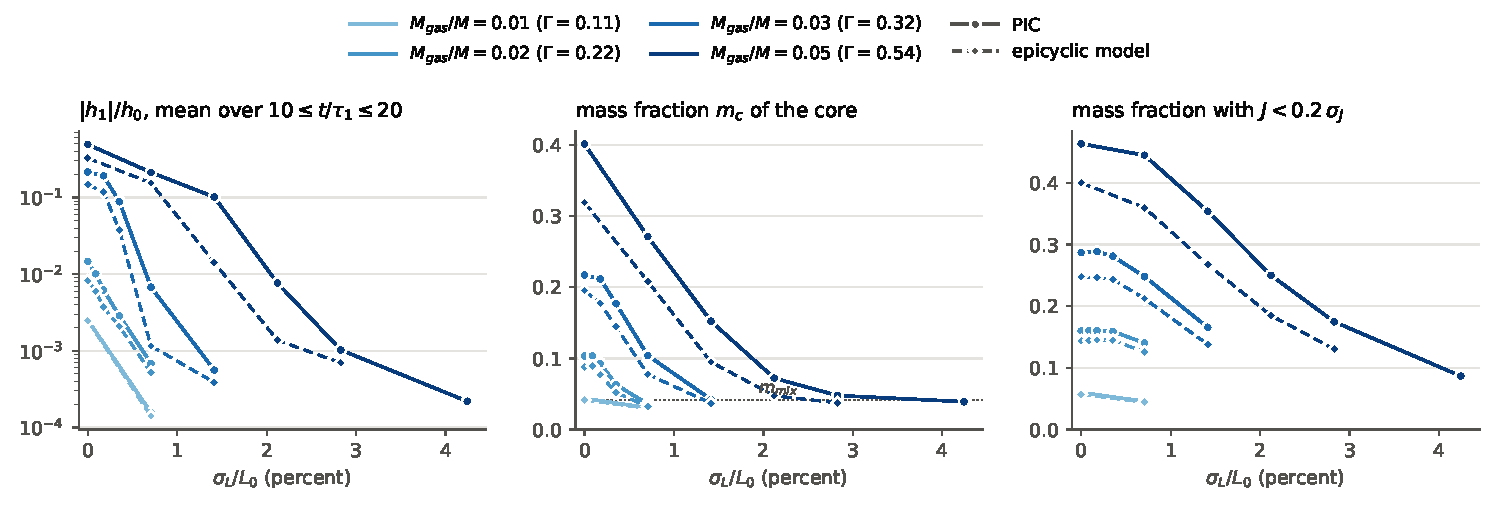
\includegraphics[width=\textwidth]{figuras/bulto_L.pdf}}
\caption{The cloud~(\ref{Eq:Pulse}) with distributed angular momenta as a function of the width $\sigma_L$ of the distribution, for four masses of the gas: PIC simulations (solid lines) and epicyclic model with the same particles (dashed lines). The quantities are those of Table~\ref{Tab:DistL}; the dotted line indicates $m_{mix}$.}
\label{Fig:DistL}
\end{figure}

Figure~\ref{Fig:DistL} and Table~\ref{Tab:DistL} show the results. For $M_{gas}/M = 0.03$ ($\mu = 0.52$), which for equal angular momenta leaves a core with $22$ percent of the mass whose oscillation persists, a width $\sigma_L/L_0 = 0.18$ percent leaves the results unchanged ($m_c = 0.212$ instead of $0.217$). For $0.35$ percent the core contains $18$ percent of the mass, and for $0.71$ percent $10$ percent, which is half of its mass for equal angular momenta; $|h_1|$ is then at least $30$ times smaller, and the residual oscillation of the potential decreases from $5.9\times 10^{-3}$ to $1.7\times 10^{-4}$, which is the level of the relaxed potentials of section~\ref{SubSec:FarRegimes}. For $1.41$ percent there is no core: $m_c = 0.042$, which is compatible with a mixed gas. The mass with $J < 0.2\sigma_J$ is reduced less: it decreases from $0.287$ to $0.248$ for $0.71$ percent and to $0.166$ for $1.41$ percent, which is still $33$ times its value without self-gravity. In the regime in which the gas mixes ($M_{gas}/M = 0.01$), a width of $0.71$ percent lowers $|h_1|$ by a factor $16$ and the mass with $J < 0.2\sigma_J$ by $24$ percent.

\begin{figure}[htp]
\centerline{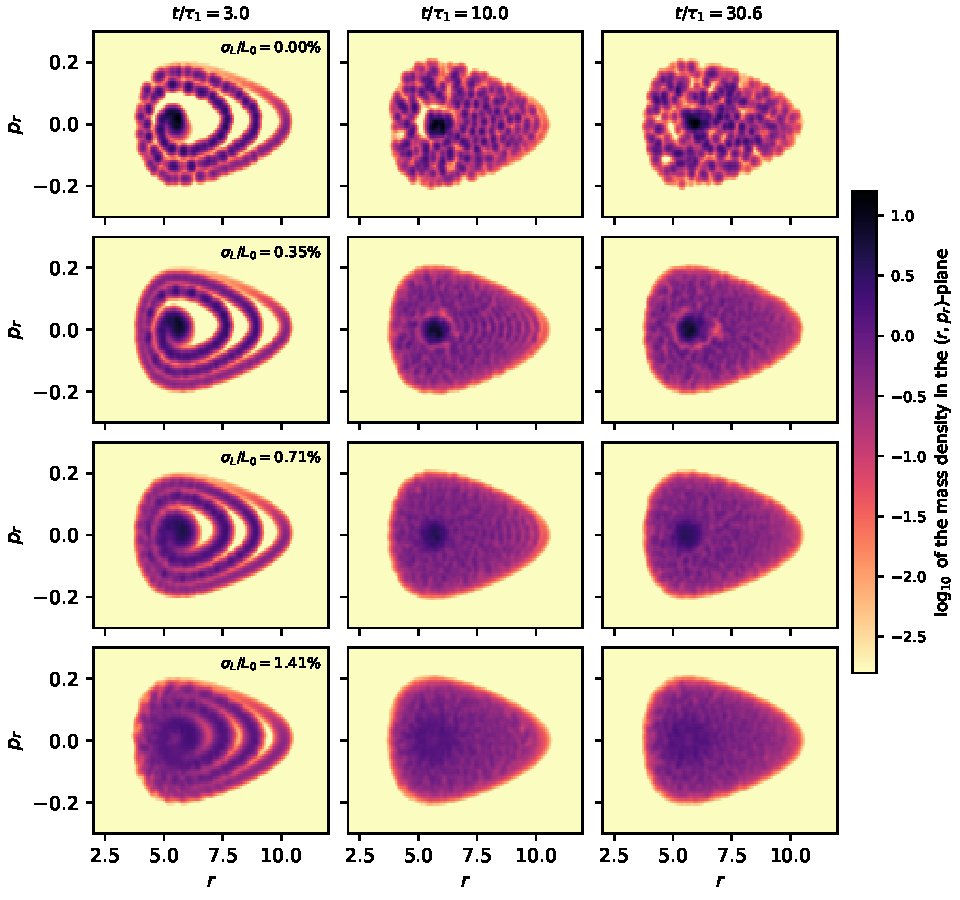
\includegraphics[width=0.85\textwidth]{figuras/bulto_L_fase.pdf}}
\caption{Density of the gas in the plane of the complex amplitude $\zeta = \sqrt{2J}\, e^{i\vartheta}$ of the radial oscillation, Eq.~(\ref{Eq:zetaDef}), for $M_{gas}/M = 0.03$ ($\mu = 0.52$) and four widths $\sigma_L$ of the distribution of the angular momenta (rows), at three times (columns). The action-angle variables are those of the instantaneous potential, computed with the angular momentum of each particle, such that the circular orbits of all the values of $L$ lie at the origin. The density is the mass of the computational particles in the cells of a grid with the spacing $0.016$, smoothed with a Gaussian kernel of the width of one cell and divided by the total mass and by the area of a cell, in logarithmic scale. The granularity of the first row is due to its small number of particles ($2100$, compared with $25\,200$, $42\,000$ and $63\,000$ in the other rows).}
\label{Fig:DistLPhase}
\end{figure}

Figure~\ref{Fig:DistLPhase} shows the same evolution in the plane of the amplitude $\zeta$ of the radial oscillation, Eq.~(\ref{Eq:zetaDef}), computed for each particle with its own angular momentum. In this plane the circular orbits of all the values of $L$ lie at the origin. In the $(r,p_r)$-plane, in contrast, the radii of the circular orbits have the root mean square spread $R'(L_0)\sigma_L$, which for $\sigma_L/L_0 = 1.41$ percent is $0.12$, comparable with the radial extension $0.14$ of the core; there, the superposition of the layers blurs the core even where each layer keeps it. At $t = 3\tau_1$ the cloud has been wound up into a spiral about the origin in all four cases; for $1.41$ percent the spiral is already smeared, since the layers with different $L$ wind up at different rates. For equal angular momenta and for $0.35$ percent a dense core remains at the origin until the end of the simulation, surrounded by a ring of low density. For $0.35$ percent the density averaged over the angle has its minimum at $|\zeta| = 0.21$ and $0.23$ at $t = 10\tau_1$ and at the end of the simulation, and the resonance~(\ref{Eq:Jres}) with the oscillation of the core lies at $(2J_{res})^{1/2} = 0.16$, at the inner edge of this ring, as the gap found in section~\ref{SubSec:EpiComparison} for equal angular momenta. For $0.71$ percent the core is fainter, and for $1.41$ percent the gas is mixed and its density has no maximum at the origin.

The layers of the lattice in $L$ show how the core is lost. For $M_{gas}/M = 0.03$, the ratio between $|h_1|$ and the mean of the values of $|h_1|$ of the individual layers, averaged over $10\leq t/\tau_1\leq 20$, is $0.99$ for $\sigma_L/L_0 = 0.18$ percent and $0.94$ for $0.35$ percent: the layers oscillate in phase. In the absence of self-gravity, the sum of their phase factors would be $\exp[-(|\partial\Omega/\partial L|\, s_L t)^2/4]$ for the Gaussian distribution at $J = 0$, which for $0.35$ percent falls from $0.22$ at $t = 10\tau_1$ to $2\times 10^{-3}$ at $t = 20\tau_1$. Hence, the gravity of the core holds the layers with different $L$ together. For $0.71$ and $1.41$ percent this ratio is $0.24$ and $0.04$, and each layer keeps a value of $|h_1|$ of $2.9\times 10^{-2}$ and $1.5\times 10^{-2}$, respectively: the layers are out of phase, and the oscillation of the gas as a whole is erased by their dephasing.

The epicyclic model reproduces these results. As for equal angular momenta (section~\ref{SubSec:EpiComparison}), for $M_{gas}/M = 0.03$ it gives a mass of the core which is smaller than in the PIC simulations by $10$ to $25$ percent, and its values of $|h_1|$ are smaller, in particular for $\sigma_L/L_0 = 0.71$ percent, where the layers are less in phase than in the PIC simulation ($0.06$ instead of $0.24$), as expected from the term omitted in the model. The model also identifies the mechanism. For $M_{gas}/M = 0.03$ and $s_L = 0.02$ we have solved Eq.~(\ref{Eq:EpicyclicL}) once with the dependence on $L$ kept only in the frequency $\Omega(J,L)$, and once with it kept only in the kernel $\mathcal{G}$, on a coarser lattice in $L$ ($N_L = 10$ points in $|L - L_0|\leq 2 s_L$), on which the full model gives the same mass of the core as on the finer one. In the first case the core contains $7.8$ percent of the mass, as with both dependences, whereas in the second case it contains $19.1$ percent, as for equal angular momenta ($19.5$ percent). Hence, the core is lost because the frequencies of its layers spread, not because the interaction is softened.


\subsection{Dependence on the mass}
\label{SubSec:DistBoundary}

The width of the distribution which is needed to remove the core grows with the mass of the cloud, see Fig.~\ref{Fig:DistL}. We measure it by the value of $\sigma_L$ at which the excess $m_c - m_{mix}$ of the mass of the core over the largest value compatible with a mixed gas has fallen to half of its value for equal angular momenta, interpolating linearly between the simulations. This happens at $\sigma_L/L_0 = 0.30$, $0.58$ and $1.00$ percent for $M_{gas}/M = 0.02$, $0.03$ and $0.05$, respectively, and at $0.26$, $0.49$ and $0.88$ percent in the model, whose cores are less resistant, as discussed above. The core is lost at $0.71$ percent for $M_{gas}/M = 0.02$, at $1.41$ percent for $0.03$, and between $1.41$ and $2.83$ percent for $0.05$. \EJ{To be narrowed with the simulation with $\sigma_L/L_0 = 2.12$ percent.} For $M_{gas}/M = 0.01$, which does not form a core, the distribution of the angular momenta only lowers $|h_1|$ and the mass near the circular orbit.

A simple estimate gives the order of magnitude of these widths, but not their dependence on the mass. The gravity of the core induces a rotation about its center with the angular velocity $g m_c M_{gas}/\rho$ at the distance $\rho$, see Eq.~(\ref{Eq:Epicyclic}), and the core should survive as long as the spread $|\partial\Omega/\partial L|\,\sigma_L$ of the frequencies of its layers is small compared with this rotation at its edge, $\rho\approx(0.1\,\sigma_J)^{1/2} = 0.1$. With the values of $m_c$ for equal angular momenta, the ratio of the two quantities at the widths found above is $0.60$, $0.37$ and $0.21$ for $M_{gas}/M = 0.02$, $0.03$ and $0.05$. Hence, the estimate locates the loss of the core at a ratio of order one, but the cores of the more massive clouds are lost at smaller ratios. The estimate treats the core as a compact object at rest at the circular orbit, whereas for $M_{gas}/M = 0.05$ its center oscillates with an amplitude of $0.44$, which exceeds its radial extension of $0.17$.

In summary, the dense core and its persistent oscillation are a property of clouds whose angular momenta are equal to within a fraction of a percent to a few percent, depending on the mass, whereas the accumulation of mass near the circular orbits survives larger widths. When the core is lost, the gas mixes and the potential which it generates relaxes. This is relevant for the setting of Ref.~\cite{sCjL26}, in which the angular momenta of the gas are distributed over an interval bounded away from zero: for such data, our results suggest that the phase space mixing proven there for small data persists for larger masses than for clouds with equal angular momenta, although our clouds extend to the circular orbit, which is excluded there.
